%%&program=xelatex
%&encoding=UTF-8 Unicode
% SVN keywords
% $Author: bernardo $
% $Date: 2014-10-24 15:26:00 +0100 (Fri, 24 Oct 2014) $
% $Revision: 6732 $
% $URL: http://metis.ipfn.ist.utl.pt/svn/cdaq/Users/Bernardo/Aulas/LFEB/teXfiles/ContrucoesGeometrica/ConstrucoesGeomet.tex $
\documentclass[a4paper,12pt]{article}      % Comments after  % are ignored
%\usepackage{hyperref}                 % For creating hyperlinks in cross references
%
%MUDAR procedimento lente divergente + angulo de Brewster
\usepackage{ifxetex}% for XELATEX, or PDFlatex
\usepackage{ifplatform} 
%
\ifxetex
	\usepackage{polyglossia} \setmainlanguage{portuges}
	\usepackage{fontspec}
	\ifwindows
		\setmainfont[Ligatures=TeX]{Garamond}
		\setsansfont[Ligatures=TeX]{Gill Sans MT}
		\setmonofont{Consolas}		
%		\setmonofont[Scale=MatchLowercase]{Courier}
	\fi
	\iflinux
		\setmainfont[Ligatures=TeX]{Linux Libertine O}
		\setsansfont[Ligatures=TeX,Scale=MatchLowercase]{Linux Biolinum}
		\setmonofont[Scale=MatchLowercase]{Courier}
	\fi
	\ifmacosx
	% add settings
	% Use xelatex -no-shell ...
		\setmainfont[Ligatures=TeX]{Garamond}
		\setsansfont[Ligatures=TeX]{Helvetica}
		\setmonofont{Consolas}
	\fi
	\usepackage{xcolor,graphicx} 
\else
	\usepackage[portuguese]{babel}
	%\usepackage[latin1]{inputenc}
	\usepackage[utf8]{inputenc}
	\usepackage[T1]{fontenc}
	\usepackage{graphics}                 % Packages to allow inclusion of graphics
	\usepackage{color}                    % For creating coloured text and background
\fi

\usepackage{enumitem}
\setlist{nolistsep}

\usepackage{tikz}
%\usetikzlibrary{calc,arrows,decorations.pathmorphing,intersections}


\usepackage{amsmath,amssymb,amsfonts} % Typical maths resource packages
\usepackage[retainorgcmds]{IEEEtrantools}

\oddsidemargin 0cm
\evensidemargin 0cm

\pagestyle{myheadings}         % Option to put page headers
                               % Needed \documentclass[a4paper,twoside]{article}

\markboth{{MEFT}}
{{\small\it \protect\input{../../LIFE.txt}}}

\addtolength{\hoffset}{-0.5cm}
\addtolength{\textwidth}{2.5cm}
\addtolength{\topmargin}{-1.5cm}
\addtolength{\textheight}{3cm}

%\textwidth 15.5cm
%\topmargin -1.5cm
\setlength{\parindent}{0pt}
\setlength{\parskip}{1ex  plus  0.5ex  minus  0.2ex}
%\parindent 0.5cm
%\textheight 25cm
%\parskip 1mm


% Math macros
\newcommand{\ud}{\,\mathrm{d}} 
\newcommand{\HRule}{\rule{\linewidth}{0.5mm}}

\author{Prof. Bernardo B. Carvalho} 

%%%%, Bernardo Brotas Carvalho\\bernardo@ipfn.ist.utl.pt} 
\date{ Outubro 2012} 

\begin{document} 

	
\includegraphics[width=0.2\textwidth]{../../logo-ist}%\\[1cm]  %%  Logo_IST_color

	\HRule \\[0.5cm]
	{ \huge \sf  \textsc{Instrumentos Ópticos Simples e \\ Goniómetro}} \\[0.4cm] % \bfseries 
%	{ \huge \sf  \textsc{Sistemas ótipos baseados em Lentes Delgadas e aproximação paraxial} }\\[0.4cm] % \bfseries 
%	{ \large \bfseries Construções Geométricas em Lentes Delgadas %(aproximação paraxial)}\\
%	{ \large \bfseries Procedimento Experimental}\\
	\HRule \\%[0.5cm]

%\newpage
\section{\sf Introdução}
Pretende-se com este trabalho desenhar e realizar no laboratório montagens ou sistemas ópticos compostos com duas ou mais lentes delgadas, testando as suas características principais. As duas montagens -- um telescópio simples e um microscópio -- são variações do esquema óptico apresentado na Secção 5 do Trabalho de Óptica Geométrica. 

Nestes sistemas, designamos por \emph{objetiva} a lente que está do lado do objeto e por \emph{ocular} aquela que está do lado do observador, com distâncias focais $f_{obj}$ e $f_{ocu}$ respetivamente. Em ambos os casos, a ocular está  próxima da \emph{imagem intermédia} A'B' formada pela objetiva. Sendo a distância inferior à distância focal $f_{ocu}$, a imagem final será \emph{virtual}, ou seja, visível apenas através da lente.\footnote{Cf. \emph{Guia de Óptica Geométrica}, Secção 3.5.}
Assim, o papel da ocular consiste em ampliar a imagem intermédia, tal como um lupa amplia um objeto.
 Continua-se neste trabalho a usar a análise da óptica geométrica paraxial ou de 1.ª ordem.


Como segundo objetivo, pretende-se que os alunos tomem conhecimento e aprendam a manusear e a tomar medidas corretamente  com um instrumento óptico de precisão, o \emph{goniómetro}. Este instrumento permite medir ângulos de desvio, por reflexão ou refração de feixes de raios paralelos, com uma resolução inferior a um minuto de grau.

\subsection{\sf O olho humano}

\begin{figure}
	[!htb]  \centering 
	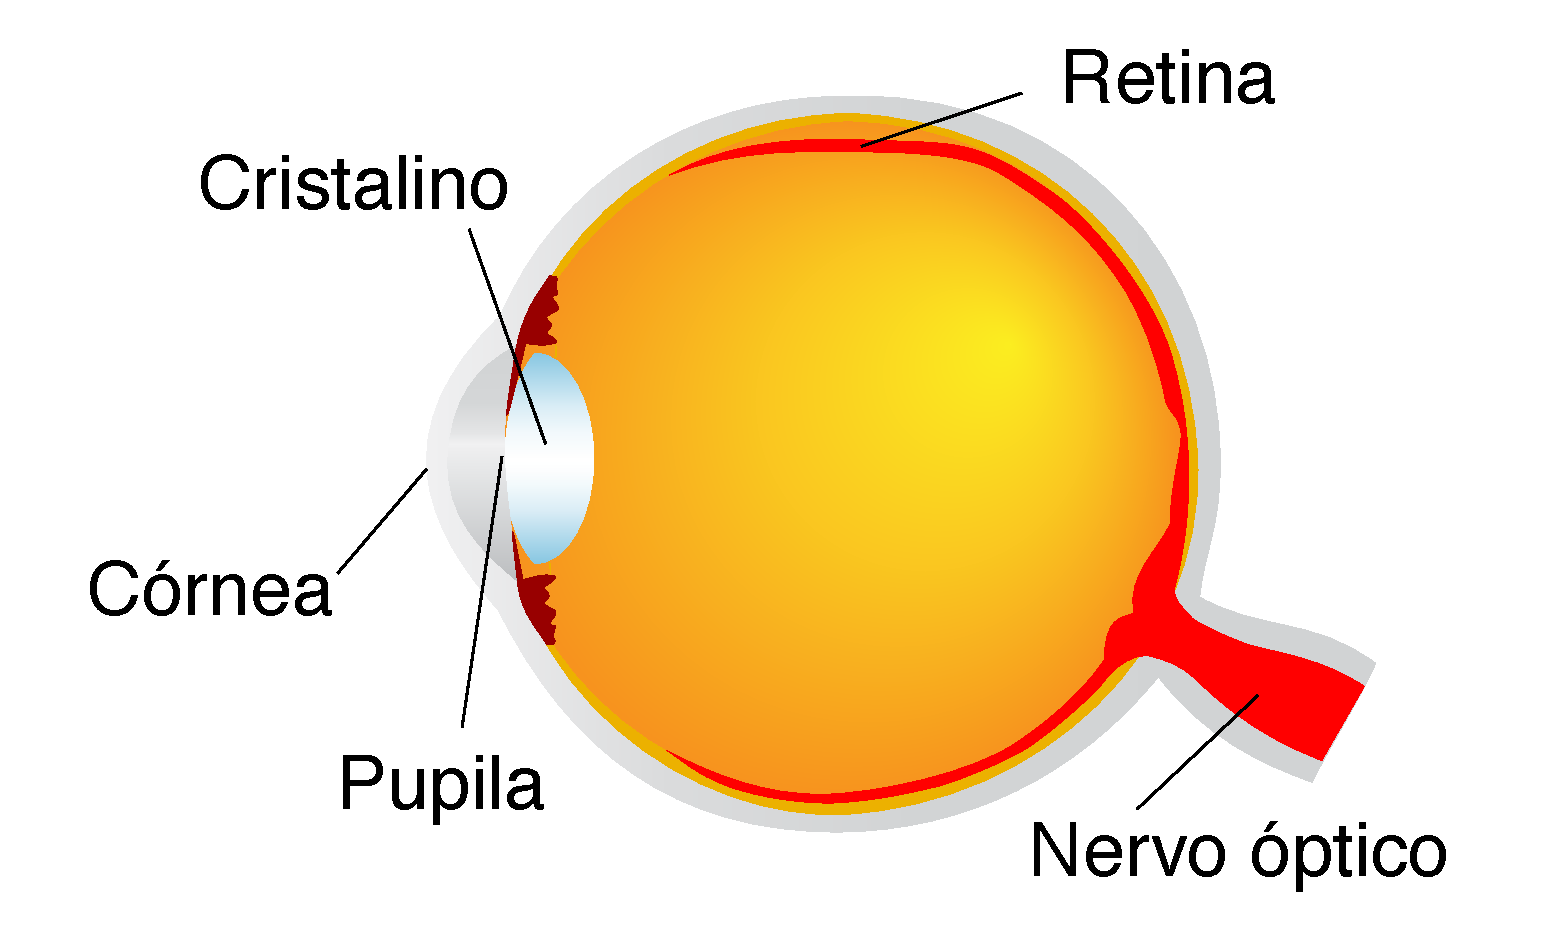
\includegraphics[width=0.5\textwidth]{olho-1}
	\caption{Diagrama dos principais elementos do olho humano. \label{fig:olho-1}} 
\end{figure}

O objectivo dos instrumentos ópticos é auxiliar a visão humana, pelo que vamos primeiro abordar a fisiologia do olho humano (Fig. \ref{fig:olho-1}). Este pode ser considerado como um sistema óptico que projecta imagens (reais) dos objectos exteriores na retina, através de duas lentes convergentes: a córnea e o cristalino. Para o nosso estudo, vamos considerar que estas lentes são substituídas por um sistema equivalente constituído por uma única lente, com o máximo de distância focal $f$ igual a 2,5 cm, que é a média da distância entre a córnea e a retina. A potência em dioptrias (dt) desta lente equivalente é dada por:

\begin{equation}
D=\frac{1}{f} \,[\mathrm{m}^{-1}] = \frac{1}{0,025} \,[\mathrm{m}^{-1}] = 40 \,[\mathrm{m}^{-1}]=40\, \mathrm{dt}.
\end{equation}


Para uma pessoa com visão normal ou munida de correção adequada (óculos graduados ou lentes de contacto), os raios ópticos provenientes de um objecto no infinito\footnote{Para efeitos práticos, considera-se o infinito óptico qualquer distância superior a 5 m.} chegam paralelos ao olho e são focados na retina sem necessidade de esforço, ou seja, com o olho relaxado (Fig. \ref{fig:olho-2} à esq.). À medida que o objecto se aproxima do olho, é necessário os músculos ciliares aumentarem a curvatura da lente para criar uma imagem focada na retina -- a isto chama-se \emph{acomodação do olho}. O ponto mais próximo do olho para o qual a lente ainda consegue focar a imagem na retina é designado por \emph{ponto próximo} (Fig. \ref{fig:olho-2} à dir.). Esta distância aumenta com a idade e considera-se o ponto próximo igual a 0,25 m para uma visão normal padrão.

\begin{figure}
	[!htb]  \centering 
	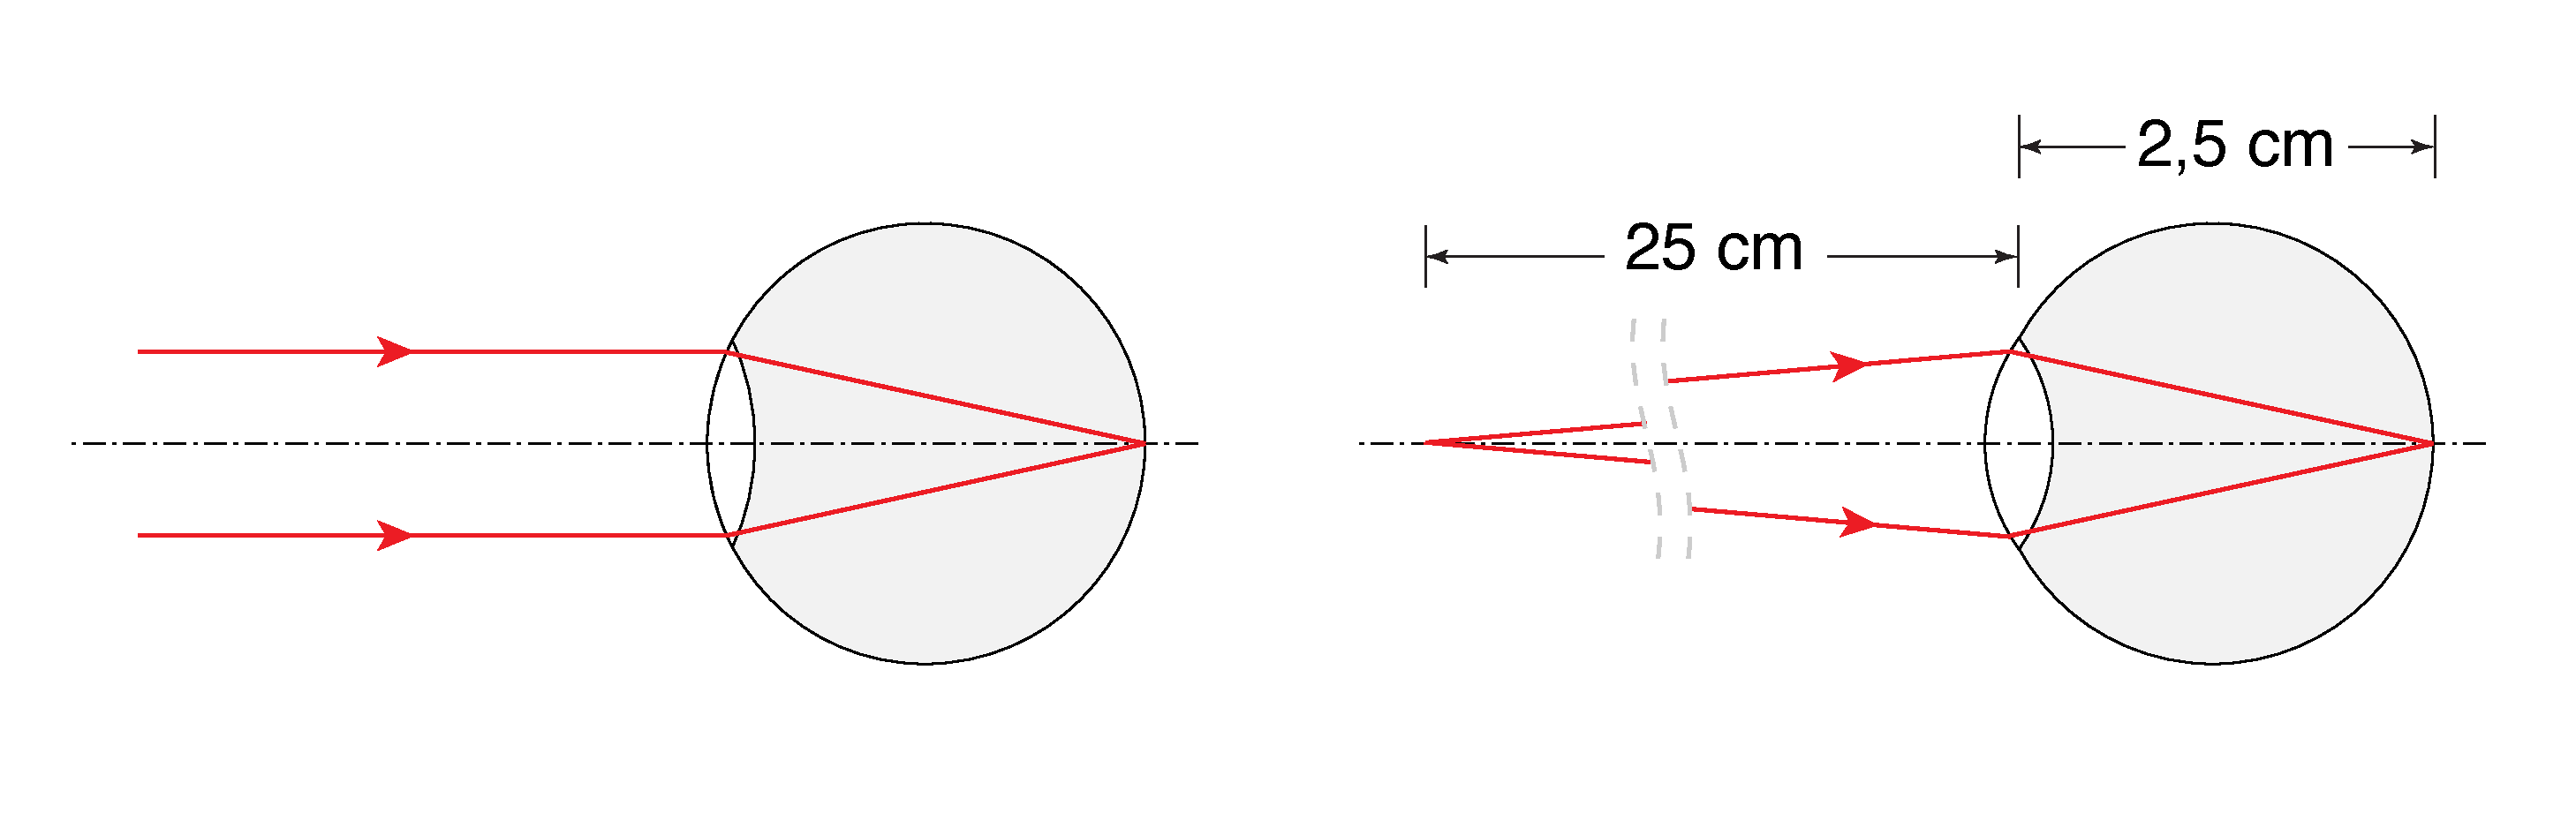
\includegraphics[width=0.9\textwidth]{olho-2}
	\caption{Esquema do olho no caso de objectos no infinito (esq.) e no ponto próximo (dir.). \label{fig:olho-2}} 
\end{figure}

O tamanho aparente dum objecto é determinado pelo tamanho que a imagem apresenta na retina. Mesmo sem variar o tamanho real do objecto, este pode ser visto maior se o aproximarmos do olho, porque o tamanho da sua imagem na retina é maior. A avaliação do tamanho da imagem na retina pode ser feita através da medição do ângulo $\theta$, que corresponde à inclinação dos raios principais do extremo da imagem (Fig. \ref{fig:olho-3}).

Considere-se um objecto com altura $h$ a uma distância $s$ do olho. Para o objeto podemos escrever $\tan\theta=h/s$. Para a imagem na retina, de altura $y'$, vem $\tan\theta = y' /$(2,5 cm). Na aproximação paraxial, ou seja de ângulos pequenos, podemos usar $\tan\theta \approx\theta$, e assim $\theta\approx h/s=y'/$(2,5 cm). Desta relação conclui-se que $y'$ é proporcional a $h$, tamanho do objecto, e inversamente proporcional à distância $s$ entre o objecto e o olho. 

\begin{figure}
	[!htb]  \centering 
	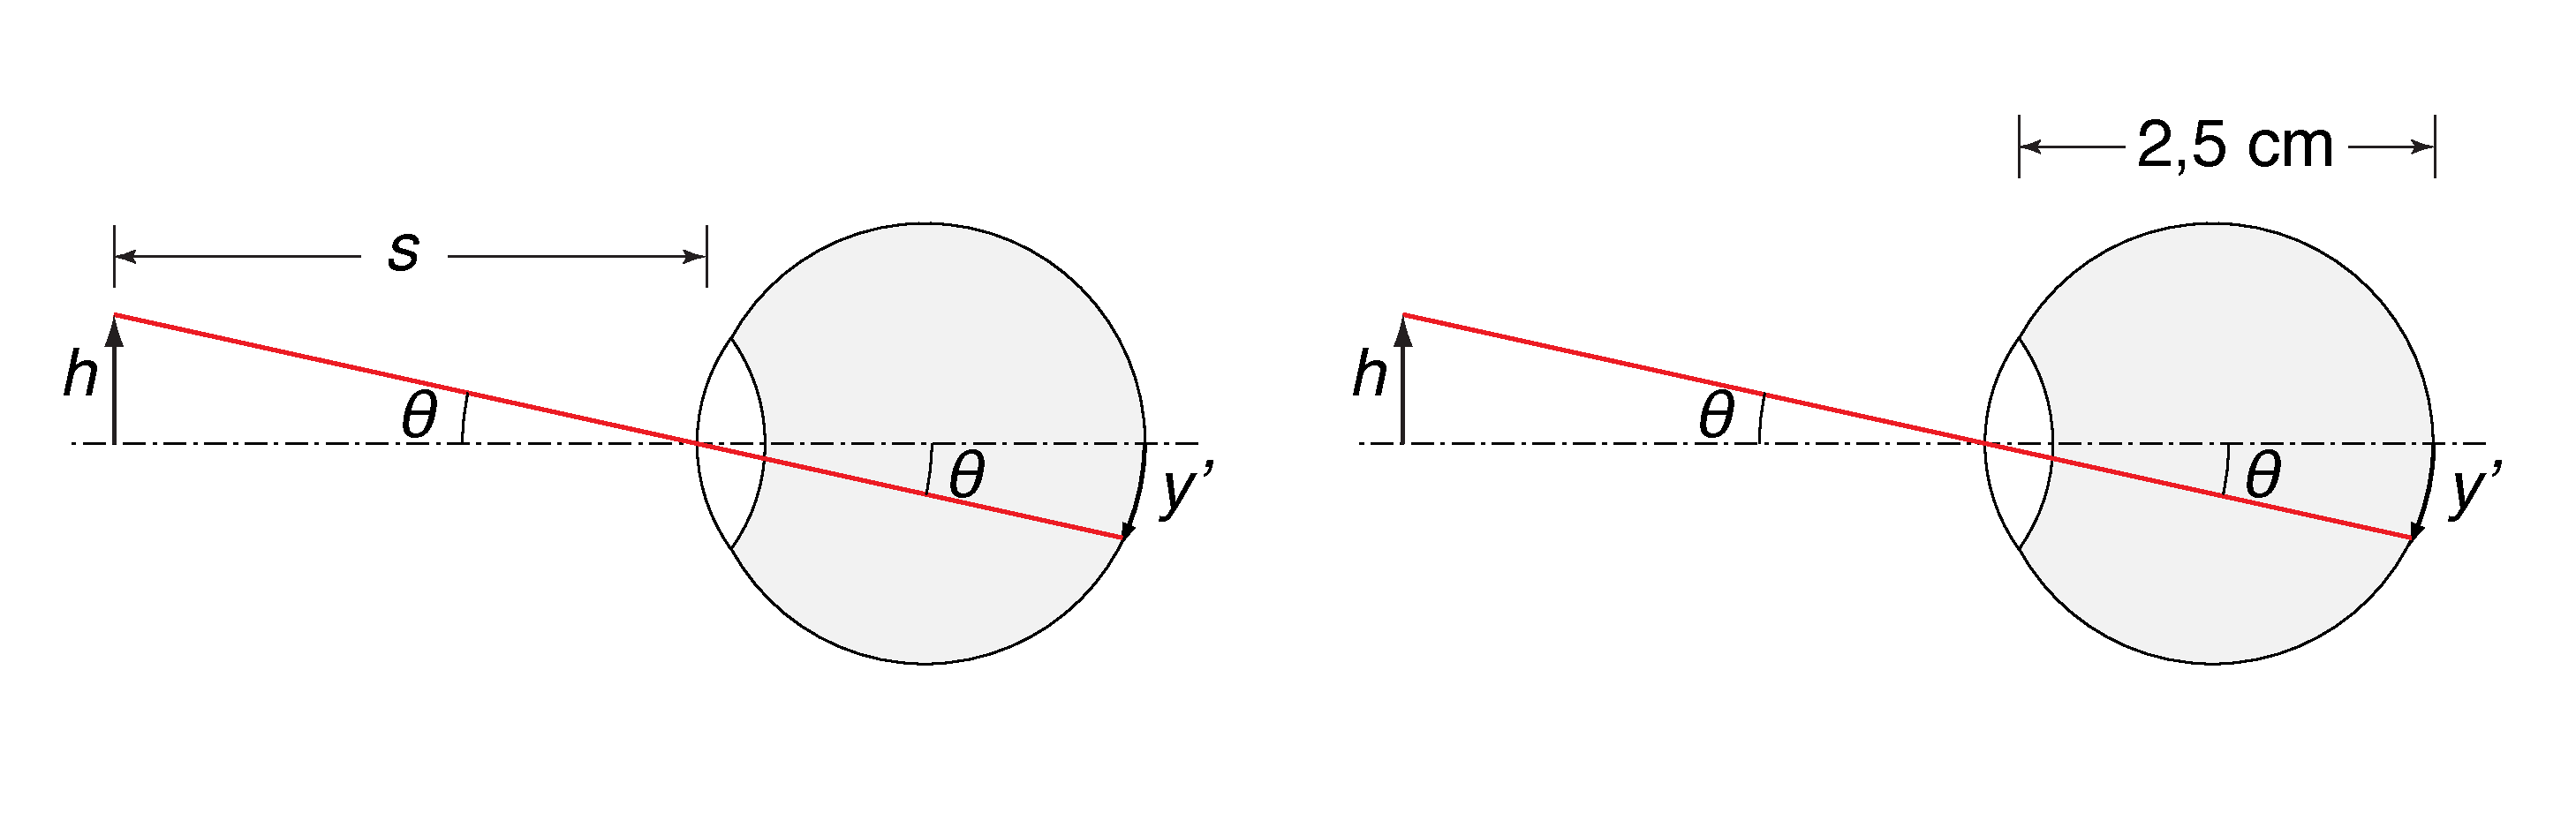
\includegraphics[width=0.9\textwidth]{olho-3}
	\caption{Formação de imagem na retina de um objecto de altura $h$ a uma distância $s$. \label{fig:olho-3}} 
\end{figure}

O princípio dos instrumentos ópticos consiste no aumento do tamanho da imagem na retina, $y'$, permitindo assim visualizar objectos muito pequenos ou afastados. Do exposto acima, podemos concluir que a sua operação baseia-se na criação de uma imagem (real ou virtual) com um tamanho aparente maior que $h$ e/ou 
 a uma distância aparente inferior a $s$. Em qualquer dos casos, a imagem final produzida deverá estar situada além do ponto próximo, caso contrário não conseguirá ser focada.






%%%%%%%%%%%%%%%%%%%%%%%%%%%%%%%%%%%%%%%%%
\subsection{\sf Lupa}

A lupa simples é o instrumento óptico mais elementar. Consiste numa só lente convergente e permite aumentar o tamanho aparente do objecto, ou seja, o tamanho da imagem na retina. Sabendo que a maior imagem que se pode obter dum objecto com o olho desarmado é quando o objecto está no ponto próximo (Fig. \ref{fig:olho-4}), e dado que $y'_0$, tamanho da imagem na retina, é proporcional ao ângulo definido entre a altura do objecto $h_0$ e a sua distância ao olho, pode-se escrever a relação

\begin{equation}
\theta_0=h_0/0,25
\end{equation}

Na visão auxiliada pela lupa, esta é colocada perto do olho, e o objecto colocado a uma distância inferior ao foco. A imagem produzida pela lupa é virtual, ampliada e direita.

\begin{figure}
	[!htb]  \centering 
	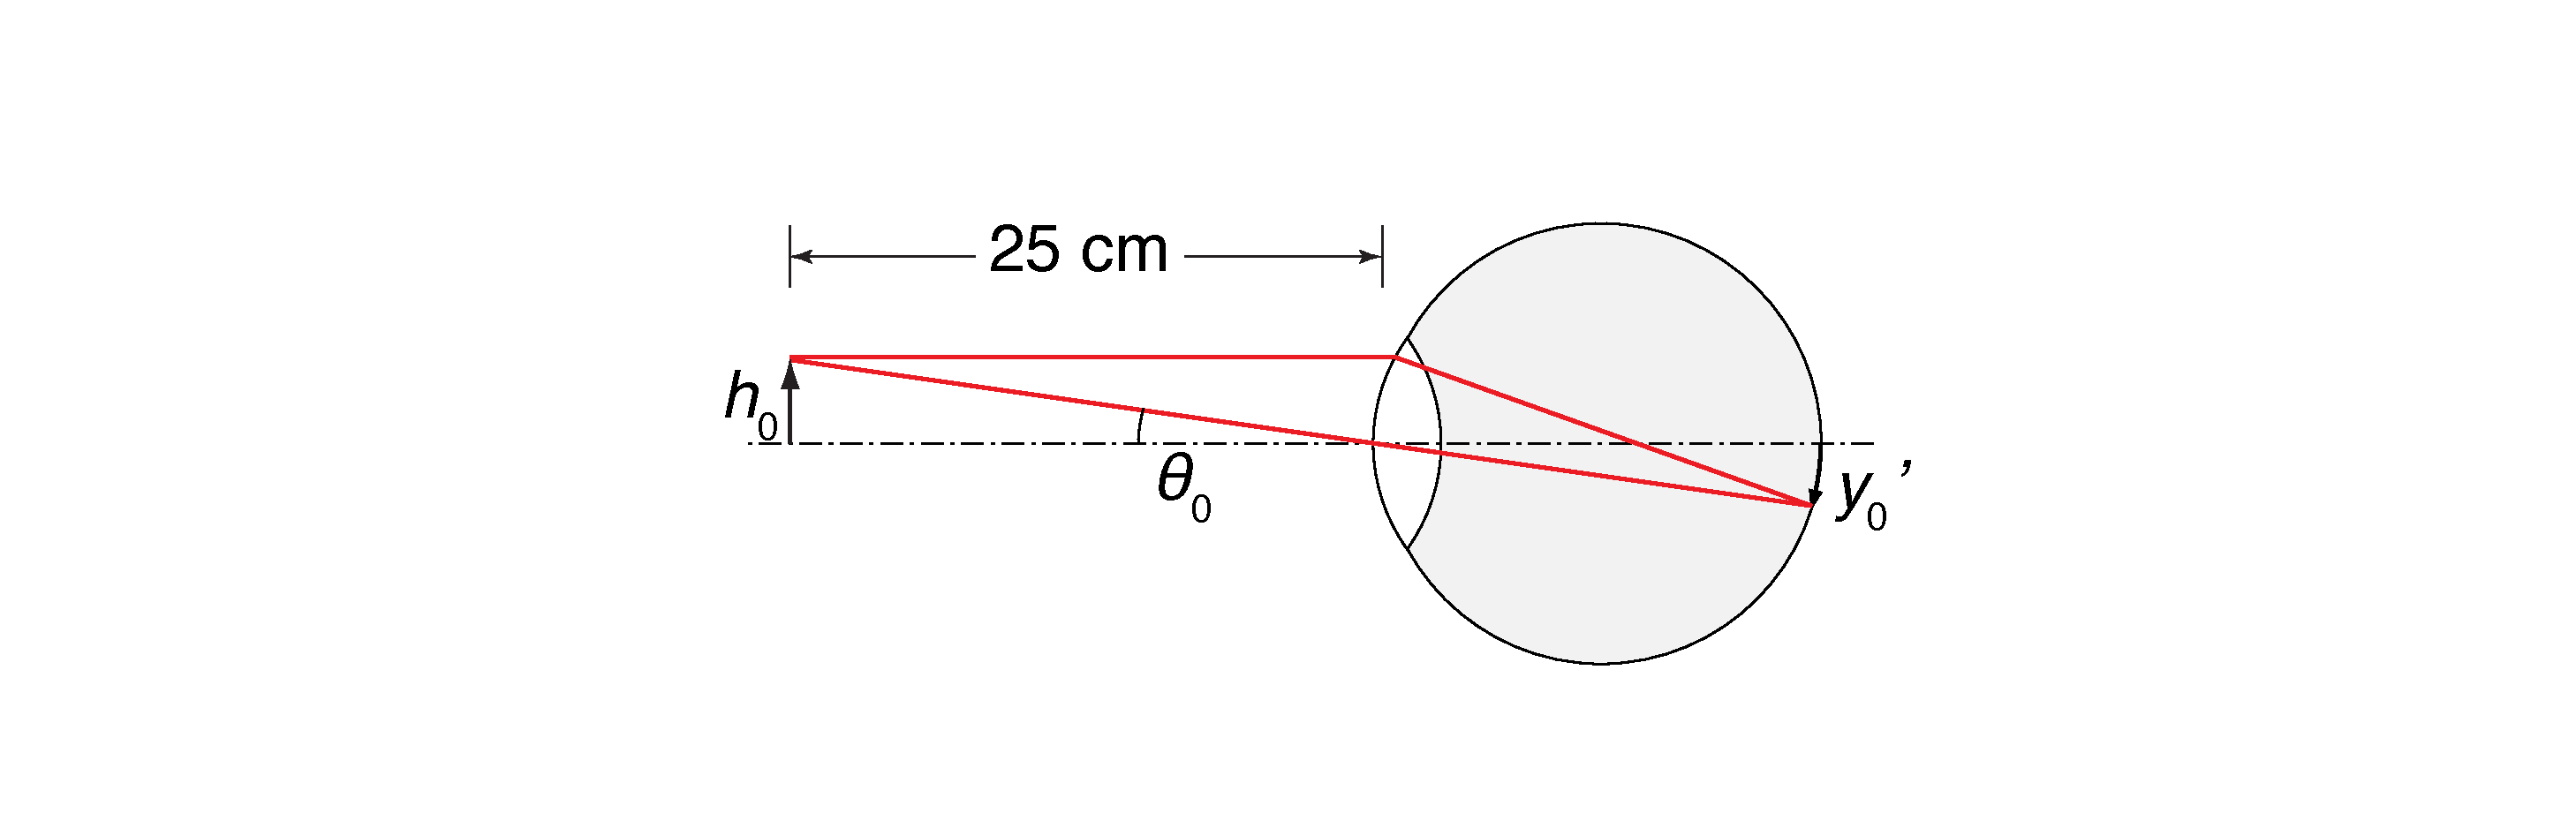
\includegraphics[width=0.8\textwidth]{olho-4}
		\caption{Objecto no ponto próximo visto pelo olho desarmado. \label{fig:olho-4}} 
\end{figure}



\begin{figure}
	[!htb]  \centering 
	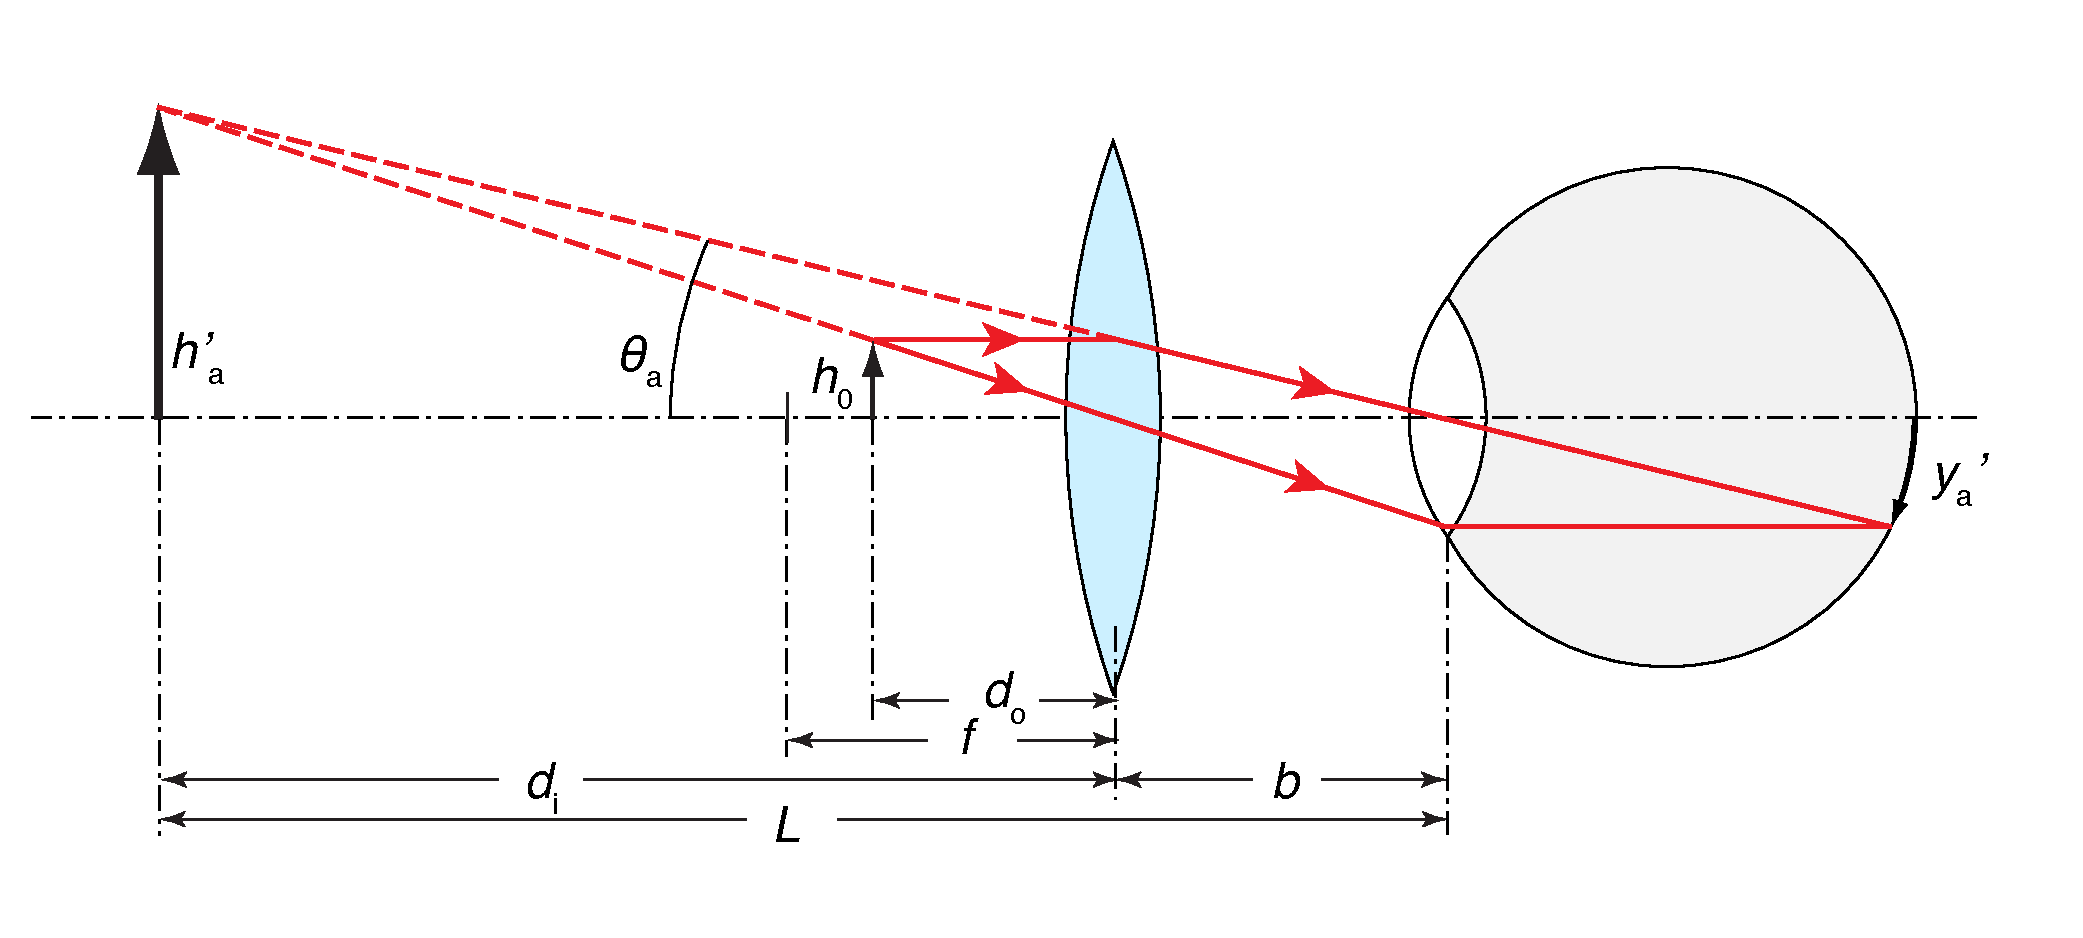
\includegraphics[width=0.8\textwidth]{olho-5}
	\caption{Formação de imagem com o auxílio de uma lupa a uma distância $b$ do olho. O objecto $h_0$ está a uma distância $d_O<f$ da lente, e a imagem (virtual) $h'_a$ aparenta estar a uma distância $d_i$ da lente e $L$ do olho. \label{fig:olho-5}} 
\end{figure}

\subsubsection{ Ampliação angular}

A \emph{ampliação angular} $M_A$ dum instrumento óptico é determinada pela razão entre $y'_a$, dimensão da imagem na retina quando o objecto é visto através do instrumento (Fig. \ref{fig:olho-5}), e $y'_0$, dimensão da imagem na retina quando vista pelo olho desarmado e o objecto no ponto próximo. A razão entre os respectivos ângulos permite esse cálculo, isto é 

\begin{equation}
M_A=\frac{y'_a}{y'_0}=\frac{\theta_a}{\theta_0}
\end{equation}

Tirando partido da aproximação paraxial, temos $\tan\theta_a = h'_a / L \approx \theta_a$ e $\tan\theta_0 = h_0 / 0,25 \approx\theta_0$, portanto pode-se escrever a ampliação angular como:

\begin{equation}
M_A = \frac{h'_a/L}{h_0/0,25}=-\frac{d_i\,0,25}{d_0 L}= \frac{0,25}{L}\left(1-\frac{d_i}{f}\right) 
\end{equation}

onde na última igualdade se recorreu à equação dos focos conjugados. Como a distância à imagem é negativa, $d_i = - (L – b)$, obtém-se por fim

\begin{equation}
M_A = \frac{0,25}{L}\left(1+\frac{L–b}{f}\right)
\end{equation}

Da análise desta expressão pode-se dizer que a ampliação diminui se $L$ ou $b$ aumentam. Existem três casos particulares de ampliação:

\begin{enumerate}

\item  Se $b=f \to M_A = \frac{0,25}{f}=0,25D$, em que $D$ é a potência da lupa em dioptrias.

\item  Se $b=0\to M_A = 0,25\left(\frac{1}{L}+\frac{1}{f}\right)$.
Se $b= 0$ e também $L = 0,25 $ m (valor mínimo para $L$, uma vez que a imagem também deve poder ser focada correctamente pelo olho), então obtém-se para $M_A$ o valor máximo, igual a $M_A = 1+\frac{0,25}{f}= 1+0,25D$. Este caso corresponde a ter a lupa "encostada" ao olho, e a imagem aumentada surge à distância do ponto próximo.

\item  Se o objecto é colocado no foco ($d_O=f$), então a lupa forma a sua imagem no infinito $(L = \infty)$ e a ampliação é $M_A = \lim_{L\to\infty}\frac{0,25}{L}\left(1+\frac{L–b}{f}\right)= \frac{0,25}{f}=0,25D$. Neste caso, o olho recebe raios paralelos e não necessita de fazer acomodação, o que é mais cómodo, e a ampliação apenas se reduz de uma unidade relativamente ao caso 2.
\end{enumerate}

Exemplo: uma lente com $D=10$ dioptrias tem uma distância focal $f=10$ cm, e para $L=\infty$ tem uma ampliação de $M_A=$2,5 vezes.


%%%%%%%%%%%%%%%%%%%%%%%%%%%%%%%%%%%%%%%%
\section {\sf Telescópio}
O telescópio é o instrumento óptico utilizado para observar, em geral, grandes objectos muito afastados do instrumento, procurando trazer a imagem do objecto para mais perto. O tipo de telescópio que vamos construir é composto por duas lentes convergentes: a lente objectiva tem distância focal $f_{obj}$ maior que a distância focal $f_{ocu}$ da lente ocular (Fig. 5). Esta montagem, designada \textit{telescópio refractor}, foi demonstrada por Galileu Galilei.

\begin{figure}
	[!htb]  \centering 
	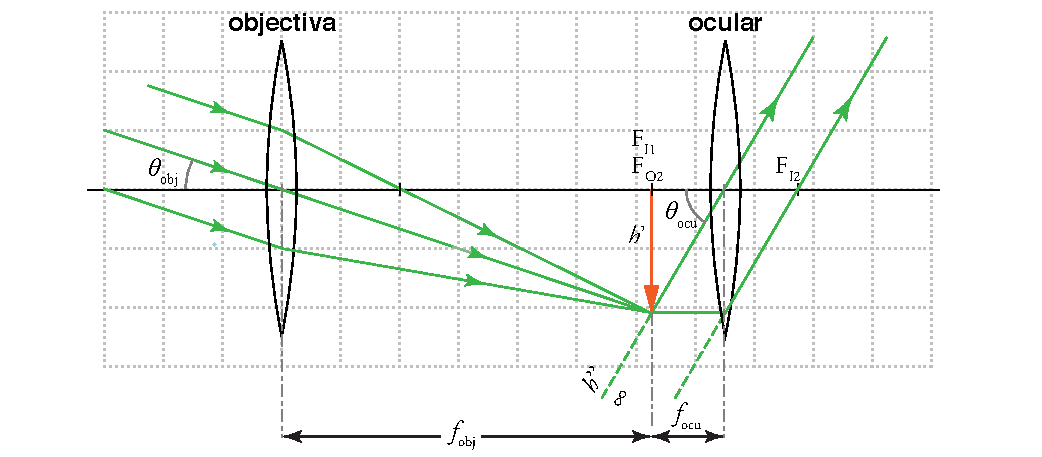
\includegraphics[width=0.95\textwidth]{telescopio2}
		\caption{Formação de imagem num telescópio. \label{fig:telescopio2}} 
\end{figure}

A objectiva vai produzir uma imagem real, invertida e localizada no foco $f_{obj}$, dado que o objecto está no infinito. Esta imagem é muito mais pequena do que o objecto e a finalidade da objectiva não é de aumentar, mas apenas de produzir uma imagem perto do observador que deve coincidir com o foco, $f_{ocu}$ da lente ocular. Assim, as lentes estão separadas de uma distância igual a $f_{obj} + f_{ocu}$.

A ampliação de um telescópio é apenas a ampliação angular dada pela razão do ângulo $\theta_{obj}$ definido pelo objecto e do ângulo $\theta_{ocu}$ definido pela imagem final. Usando a aproximação paraxial e tendo em conta que a imagem é invertida, temos
\begin{equation}
\tan\theta_{obj}= -\frac{h’}{f_{obj}} \approx \theta_{obj} \,\,\,\,\,\,\,\,\,\tan\theta_{ocu} =\frac{h’}{f_{ocu}}\approx\theta_{ocu}
\end{equation}

e portanto a ampliação final é
\begin{equation}
M=M_A =\frac{\theta_{obj}}{\theta_{ocu}}= -\frac{f_{obj}}{f_{ocu}}.
\end{equation}

\subsection{\sf Procedimento Experimental}

Material: Lente objectiva $f$ = 150 mm e ocular $f$ = 75 mm.

\begin{enumerate}
\item Na folha quadriculada em anexo desenhe um diagrama de traçado de raios, utilizando as lentes indicadas acima e considerando o objecto no infinito. Obtenha a posição da imagem intermédia (plano focal) e determine a posição da ocular que permite obter um feixe de raios paralelos (imagem no infinito).
\item Monte o esquema como indicado na Fig. \ref{fig:telescopio2}.
\item Num extremo da sala, junto à porta, aponte para a escala colocada na parede do fundo (próximo da janela).
\item Ajuste a distância entre as lentes de modo a trazer a imagem para o foco, anotando os valores medidos.
\item Para medir a ampliação, olhe com um só olho para a imagem e com o outro olho o objecto directamente.
\item Relacione os tamanhos da imagem final e do objecto e compare com a ampliação teórica.
\end{enumerate}


%%%%%%%%%%%%%%%%%%%%%%%%%%%%%%%%%%%%%%%%%
\section{\sf Microscópio composto}

O microscópio é o instrumento óptico empregado para observar objectos pequenos, colocados muito próximos do instrumento. Na sua forma mais simples, consiste em duas lentes convergentes. A lente mais próxima do objecto (\emph{objectiva}) tem uma distância focal $f_{obj}$, menor que a distância focal $f_{ocu}$ da lente mais perto do olho (\emph{ocular}) (Fig. \ref{fig:microscopio}).

\begin{figure}
	[!htb]  \centering 
	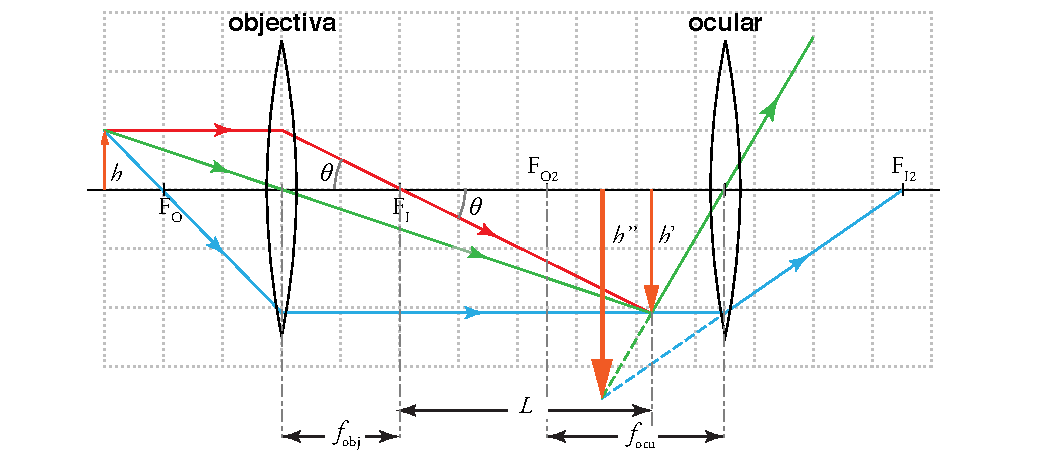
\includegraphics[width=1.0\textwidth]{microscopio}
		\caption{Formação de imagem num microscópio. \label{fig:microscopio}} 
\end{figure}

Um objecto de altura $h$ é colocado, em relação à objectiva, mais afastado do que o foco desta, produzindo uma imagem de tamanho $h'$ que é real, invertida e maior que o objecto. A objectiva produz uma imagem com \emph{ampliação transversal linear} $M_T$,\footnote{No \textit{Guia de óptica Geométrica}, para o caso de uma única lente, esta ampliação é designada $A$.} dada por:

\begin{equation}
M_T=\frac{h'}{h} = -\frac{L\tan\theta}{f_{obj}\tan\theta}= -\frac{L}{f_{obj}}
\end{equation}

O sinal negativo indica que a imagem é invertida e, uma vez que é real, a imagem pode ser projectada sobre um alvo para se medir o seu tamanho.

A lente ocular é usada para aumentar a imagem formada pela lente objectiva. Assim, a ocular é colocada de modo a que a imagem $h'$ produzida pela objectiva (agora \emph{objecto virtual} da segunda lente) venha localizar-se a uma distância ligeiramente inferior ao seu foco $f_{ocu}$. Nesta condição, a ocular actua como uma simples lupa, que permite trazer o objecto $h’$ para uma distância mais curta do que o ponto próximo (0,25 m), e produz a imagem $h''$. A \emph{ampliação final} $M$ é dada pelo produto da ampliação transversal para a lente objectiva e a ampliação angular obtida para a lente ocular. No caso da lente ocular estar encostada ao olho, como é habitual num microscópio, estamos no caso em que a distância $b=0$, e das expressões anteriores para a ampliação linear e angular obtemos

\begin{equation}
M = \frac{h''}{h}=M_T\times M_A =\frac{h’}{h}\times0,25\left(\frac{1}{L}+\frac{1}{f_{ocu}}\right)=-\frac{1}{f_{obj}}\times0,25\left(1+\frac{L}{f_{ocu}}\right).
\end{equation}


\subsection{\sf Procedimento Experimental}

Material: Lente objectiva $f$ = 75 mm e ocular $f$ = 150 mm.

\textbf{Medição da ampliação angular da ocular}
\begin{enumerate}
\item Monte um ecrã graduado (E1) na parte lateral exterior de um suporte a 25 cm da extremidade da calha, de modo a ficar no ponto próximo do observador. Esta será a \emph{escala de referência}, desempenhando o mesmo papel que a escala na parede, no caso do telescópio.
\item Monte a lente ocular junto à mesma extremidade da calha, de modo a obter a condição $b\sim 0$ (verifique a Fig. \ref{fig:olho-5}). Calcule qual a distância dessa lente a que deverá colocar um objecto de modo a que a sua imagem surja no ponto próximo. Use o valor obtido para determinar a ampliação angular (calculada).
\item Coloque outro ecrã graduado (E2) próximo da posição calculada (entre a lente e o ecrã E1), de modo a conseguir visualizar simultaneamente (a) a escala de E2 através da lente, com o olho esquerdo, e (b) a escala de E1 com o olho direito, directamente. 
\item Ajuste a posição de E2 até conseguir focar simultaneamente as imagens em ambos os olhos. Sobrepondo visualmente as escalas das duas imagens, meça o tamanho aparente da imagem (virtual) de E2 e determine a ampliação angular da lente, usando a expressão adequada para esta configuração.
% \item Na folha quadriculada em anexo desenhe um diagrama de traçado de raios, com o objecto a uma distância do foco igual $\approx f/5$. Obtenha a posição da imagem intermédia e da imagem final.
\end{enumerate}

\textbf{Medição da ampliação linear da objectiva}
\begin{enumerate}[resume]
\item Mantendo a ocular numa extremidade, monte o esquema como indicado na Fig. \ref{fig:microscopio}, usando como objecto um écran graduado iluminado.
\item Se necessário, ajuste a objectiva de modo a observar uma imagem focada através da ocular.
\item Projecte sobre outro ecrã a imagem intermédia  $h’$ bem focada e meça a sua ampliação.
\item Calcule a ampliação final do microscópio composto.
\end{enumerate}






%%%%%%%%%%%%%%%%%%%%%%%%%%%%%%%%%%%%%%%%
\section{\sf Goniómetro de Babinet}
O goniómetro é um instrumento que permite medir ângulos com grande precisão, e muito utilizado em óptica. O goniómetro de Babinet tem uma base central quase cilíndrica com uma plataforma que roda em torno do eixo vertical daquela, na qual é colocado o prisma (ou a rede de difração) a caracterizar (Figura \ref{fig:goniometer}). 

O goniómetro vem equipado com dois elementos ópticos: um \emph{colimador} e uma \emph{luneta}. Ambos estão montados radialmente, o colimador fixo e a luneta podendo rodar em torno do eixo da base (Figura \ref{fig:babinet}). As posições angulares da plataforma (e portanto do prisma) e da luneta podem ser lidas num limbo graduado por intermédio de nónios solidários, respetivamente com a plataforma e a luneta. Existem dois parafusos micrométricos, cada um associado a cada um dos nónios, que permitem com facilidade regular e fazer leituras das posições angulares, com resolução de $30''$ (meio minuto de grau).

\begin{figure}[htb]  
\centering 
	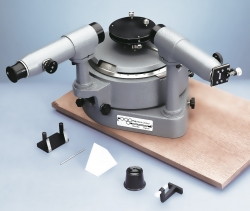
\includegraphics[width=0.45\textwidth]{goniometer}
	\caption{Goniómetro de Babinet (modelo Philipe Harris Advanced Spectrometer 30). \label{fig:goniometer}} 
\end{figure}

O colimador é constituído por dois tubos cilíndricos concêntricos que se podem deslocar axialmente. Um deles possui uma fenda retilínea, de largura variável por um parafuso, e que deve ser colocada na vertical (pode utilizar a mira da ocular depois de regulada). O outro tubo tem no extremo oposto (mais próximo do eixo) uma lente convergente, $L_C$. O objetivo deste conjunto, quando a fenda é iluminada por uma fonte luminosa divergente, é produzir um feixe de raios paralelos na região da plataforma, onde se coloca o prisma, rede, ou espelho. A fenda, se for relativamente estreita, vai funcionar como objeto linear.

\begin{figure}[!htb]  
	\centering 
	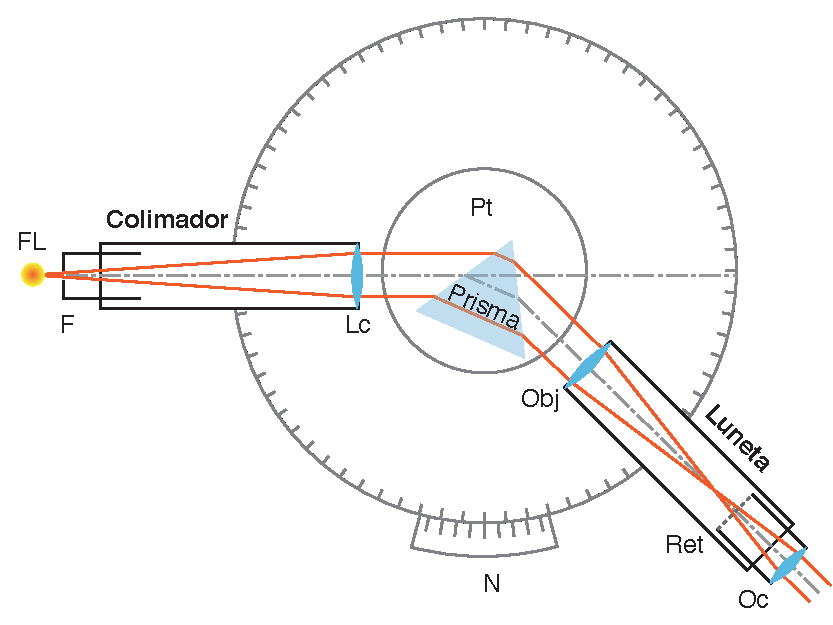
\includegraphics[width=0.65\textwidth]{Babinet}
	\caption{Esquema do Goniómetro de Babinet. Legenda: FL -- fonte luminosa, F -- fenda, Lc -- lente convergente do colimador, Pt -- plataforma, Obj -- objetiva, Oc -- ocular, Ret -- retículo, N -- nónio acoplado à luneta\label{fig:babinet}} 
\end{figure}

A luneta é constituída por dois elementos ópticos, uma lente convergente e uma ocular munida de retículo (dois fios cruzados perpendicularmente). A primeira lente produz no seu plano focal a imagem intermédia da fenda, que é projetada no plano do retículo e ampliada pela ocular. A ocular é regulada pelo observador, de modo a ver uma imagem focada da fenda. Quando se dispõe de um sistema de deteção (placa fotográfica ou um detetor, por exemplo uma célula fotoelétrica com um sistema de amplificação), este é colocado diretamente no plano focal da lente convergente e é retirada a ocular.

A regulação do instrumento pelo utilizador é feita sempre na seguinte ordem:
\begin{enumerate}
\item Focar  o retículo para um olho sem necessidade de acomodação (relaxado) e alinhá-lo com a vertical usando um fio de prumo, ou alguma linha vertical no laboratório.
\item Focar a ocular observando um objecto no infinito (ou quase).
\item Alinhar a luneta e o colimador para observar a fenda iluminada. Focar a imagem da fenda, regulando APENAS o parafuso do colimador.
\item Alinhar a fenda com a vertical, sobrepondo a mira e reduzir a sua largura para um valor suficientemente estreito, embora claramente visível.
\end{enumerate}

\bigskip
\bigskip

\fbox{\begin{minipage}{38em}
\textbf{Atenção:} este trabalho envolve o uso de lâmpadas espetrais. Estas lâmpadas são uma fonte de radiação ultravioleta, que tem efeitos nocivos nos olhos e na pele. Apesar das lâmpadas existentes no laboratório terem uma potência de emissão relativamente baixa, deve-se evitar a exposição desnecessária ou a observação prolongada da sua luz.
\end{minipage}}

\newpage
\subsection{\sf Procedimento experimental}
%\subsection{\sf Questões a responder ANTES da sessão de Laboratório:}
%\begin{enumerate}
%\item Descreva por palavras suas quais os objectivos do Trabalho que irá realizar na sessão de Laboratório (uma folha A4). Indique as expressões que irá utilizar para obter as grandezas experimentais, bem como as expressões para calcular as incertezas. Inclua esta parte também no Relatório. Este irá constituir o ÚNICO meio de consulta na Prova Individual.
	
%\item A partir da equação das lentes delgadas $\frac{1}{f} = (n_{vidro}-1) \left(\frac{1}{R_1} -\frac{1}{R_2}\right)$ e assumindo que os dois raios $R_1$ e $R_2$ das superfícies esféricas das lentes utilizadas no trabalho anterior são iguais e $ n_{vidro}=1.57$, calcule $R_{1,2}$ para todas as lentes esféricas utilizadas no trabalho de Ótica.
%\item Assumindo que o diâmetro das lentes é $D=4$ cm, calcule a sua espessura mínima. Podem ser fielmente consideradas como lentes delgadas?
%\item Como variam as distâncias focais se estas lentes forem mergulhada em água? (\emph{Sugestão: considere a forma da equação das lentes delgadas.})
%\end{enumerate}

\textbf{Material utilizado}
%1ª Parte
%\begin{itemize}
%\item caixa de ótica equipada com calha graduada
%\item lentes convergentes e divergente
%\item semi-cilindro de vidro acrílico
%\item objeto com mira
%\item diafragmas
%\item suportes
%\item fonte luminosa com lâmpada de incandescência linear
%\end{itemize}

%2ª Parte




\begin{itemize}
\item goniómetro
\item fonte de luz incandescente (candeeiro)
\item luz espetral de Hg ou He
\item prisma
\item rede de difração
\item nível graduado
\end{itemize}

%\subsection{\sf Procedimento Experimental}

%\subsubsection{\sf  Telescópio}

%A montagem  a utilizar é da Figura \ref{fig:Telescopio}, embora o objecto esteja situado a uma distância grande (> 5 m). 

%\begin{enumerate}
%\item Na folha quadriculada em anexo desenhe um diagrama de traçado de raios, utilizando como objectiva a lente mais potente do trabalho de Ótica Geométrica, e considerando o objecto no infinito. Obtenha a posição da imagem intermédia (plano focal). 
%\item Calcule agora a posição da lente ocular, com $f_{ocu}=150$ mm, para obter uma ampliação transversal entre a imagem intermédia e a imagem final de $M_T=-3$. 
%\item Utilizando as aproximações paraxial e das lentes delgadas, desenhe a construção geométrica e obtenha a posição da imagem e a respetiva ampliação.
%\item Tente montar o sistema na calha e observe um objeto distante a partir da lente ocular. Foque bem a imagem e registe a posição das duas lentes. Compare com o diagrama de traçado de raios.
%\item Calcule a o Número f do telecópio (inverso da Abertura %relativa)   a partir dos diâmetro, $D$, e distancia focal da %Objetiva, $f$. Compare com o valores das máquinas fotográficas %comerciais.
%$$f/\# \equiv \frac{}{}$$. 
%\end{enumerate}

%\subsubsection{\sf  Microscópio}

%Nesta montagem equivalente, iremos trocar a posição da lentes (objetiva/ocular) e colocar um pequeno objeto a uma distância um pouco maior que a distância focal da objetiva $f_{obj}$. A ampliação total deste sistema é o produto da ampliação transversal da objectiva, $M_{T_{obj}}$,  e da \emph{ampliação angular}\footnote{Definida como a razão entre a dimensão da imagem na retina quando o objeto é visto através da lente e a dimensão do objecto quando visto pelo olho desarmado à distância normal de observação, que é cerca de 25 cm.} da ocular, $M_{A_{ocu}}$.
 
%A ampliação transversal é calculada pela razão
%$$M_{T_{obj}}=-\frac{d_I}{d_O}=-\frac{d_I - f_{obj}}{f_{obj}}$$

%A ampliação angular pode ser estimada por 
%$$M_{A_{ocu}}= \frac{0.25}{f_{ocu}}$$

%\begin{enumerate}
%\item Na folha quadriculada em anexo desenhe um diagrama de traçado de raios, com o objecto a uma distância do foco igual $\approx f/5$. Obtenha a posição da imagem intermédia. Calcule agora a posição da lente ocular para obter um feixe de raios paralelos (imagem no infinito).
%\item Tente montar o sistema na calha e observe o slide com a mira graduada. Com auxílio do slide transparente graduado, tente estimar a ampliação do  objeto distante a partir da lente ocular. Foque bem a imagem e registe a posição das duas lentes. Compare com o diagrama de traçado de raios.
%\item Calcule a ampliação total do sistema.
%\item Identifique os vários tipos de imperfeição que pode observar na imagem. 
%\end{enumerate}

%\subsubsection{\sf Goniómetro de Babinet}


\textbf{Alinhamento do goniómetro}
\begin{enumerate}
%\item Ligue  a  lâmpada  espetral  e  espere  10  a  15  minutos    %até  que  se  estabeleça  o 
%equilíbrio térmico no seu interior. 
\item Disponha o goniómetro em frente a uma fonte luminosa de luz incandescente. Entretanto, ligue também a fonte de luz espetral, de modo a permitir que se estabilize termicamente (10 a 15 minutos).
\item Comece por regular a ocular da luneta. Para isso, deve ver nitidamente com um olho  os fios do retículo e simultaneamente com o outro olho ver um objeto no exterior da luneta, afastado a cerca de 30 cm.  
\item Para  regular  a  objetiva,  observe  agora  um  objeto  no  “infinito” (no  laboratório, escolha  um objeto o mais  afastado possível)  atuando  sobre  o  parafuso  da  luneta.  Regule  de  modo  a observar o objeto e o retículo, bem focado e sem paralaxe. 
\item Coloque  a  luneta  alinhada de frente  para o  colimador  e  regule o parafuso deste, de modo a observar a fenda focada quando iluminada pela lâmpada espetral. 
\item Com a ajuda do nível de bolha, verifique o nivelamento horizontal do goniómetro e da plataforma.
\item Identifique as escalas dos ângulos usados para medir a posição da plataforma e da luneta. Assegure-se de que compreende como estão relacionadas as duas escalas opostas antes de efectuar as medições. Qual a resolução mínima do conjunto escala/nónio?
\end{enumerate}

\textbf{Rede de difracção}


\begin{enumerate}[resume]
\item Monte no centro da plataforma do goniómetro uma rede de difração de 600 linhas por milímetro, orientada com uma das faces de frente para o colimador. Substitua a lâmpada incandescente pela fonte de luz espetral. Observe os raios \emph{difratados} de várias cores, em 1.ª e 2.ª ordem. Identifique os diversos comprimentos de onda e meça os respectivos ângulos de desvio, com a melhor precisão possível.
\end{enumerate}

\textbf{Prisma}
\begin{enumerate}[resume]
\item Substitua na plataforma a rede de difração por um prisma (de ângulo de vértice conhecido), de modo a obter uma configuração semelhante à da Figura \ref{fig:babinet}.
\item  Observe  a transmissão  das várias cores  através  do  prisma.  Se o instrumento estiver bem focado, deverá  observar  uma  série  de 
imagens coloridas da mesma fenda isoladas (riscas), uma por cada comprimento de onda.
\item Escolha duas dessas cores bem afastadas. Rodando o prisma, obtenha um conjunto de valores que permita fazer um gráfico dos ângulos de desvio $\delta(i_1)$ em função do ângulo de incidência $i_1$ e um ajuste polinomial. A partir do gráfico, verifique que existe um valor mínimo para o ângulo de desvio,  $ \delta(i_{min})$, mas  que este e o ângulo $i_{min}$ são  diferentes para cada cor.
\end{enumerate}


	
\newpage
\def\width{18}
\def\hauteur{25}
\begin{tikzpicture}[x=1cm, y=1cm, semitransparent]
\draw[step=1mm, line width=0.1mm, black!30!white] (0,0) grid (\width,\hauteur);
\draw[step=5mm, line width=0.2mm, black!40!white] (0,0) grid (\width,\hauteur);
\draw[step=5cm, line width=0.5mm, black!50!white] (0,0) grid (\width,\hauteur);
\draw[step=1cm, line width=0.3mm, black!90!white] (0,0) grid (\width,\hauteur);
\end{tikzpicture}


\end{document} 